\subsection{Klassen-Diagramm}
	\begin{figure}[H]
        \centering
        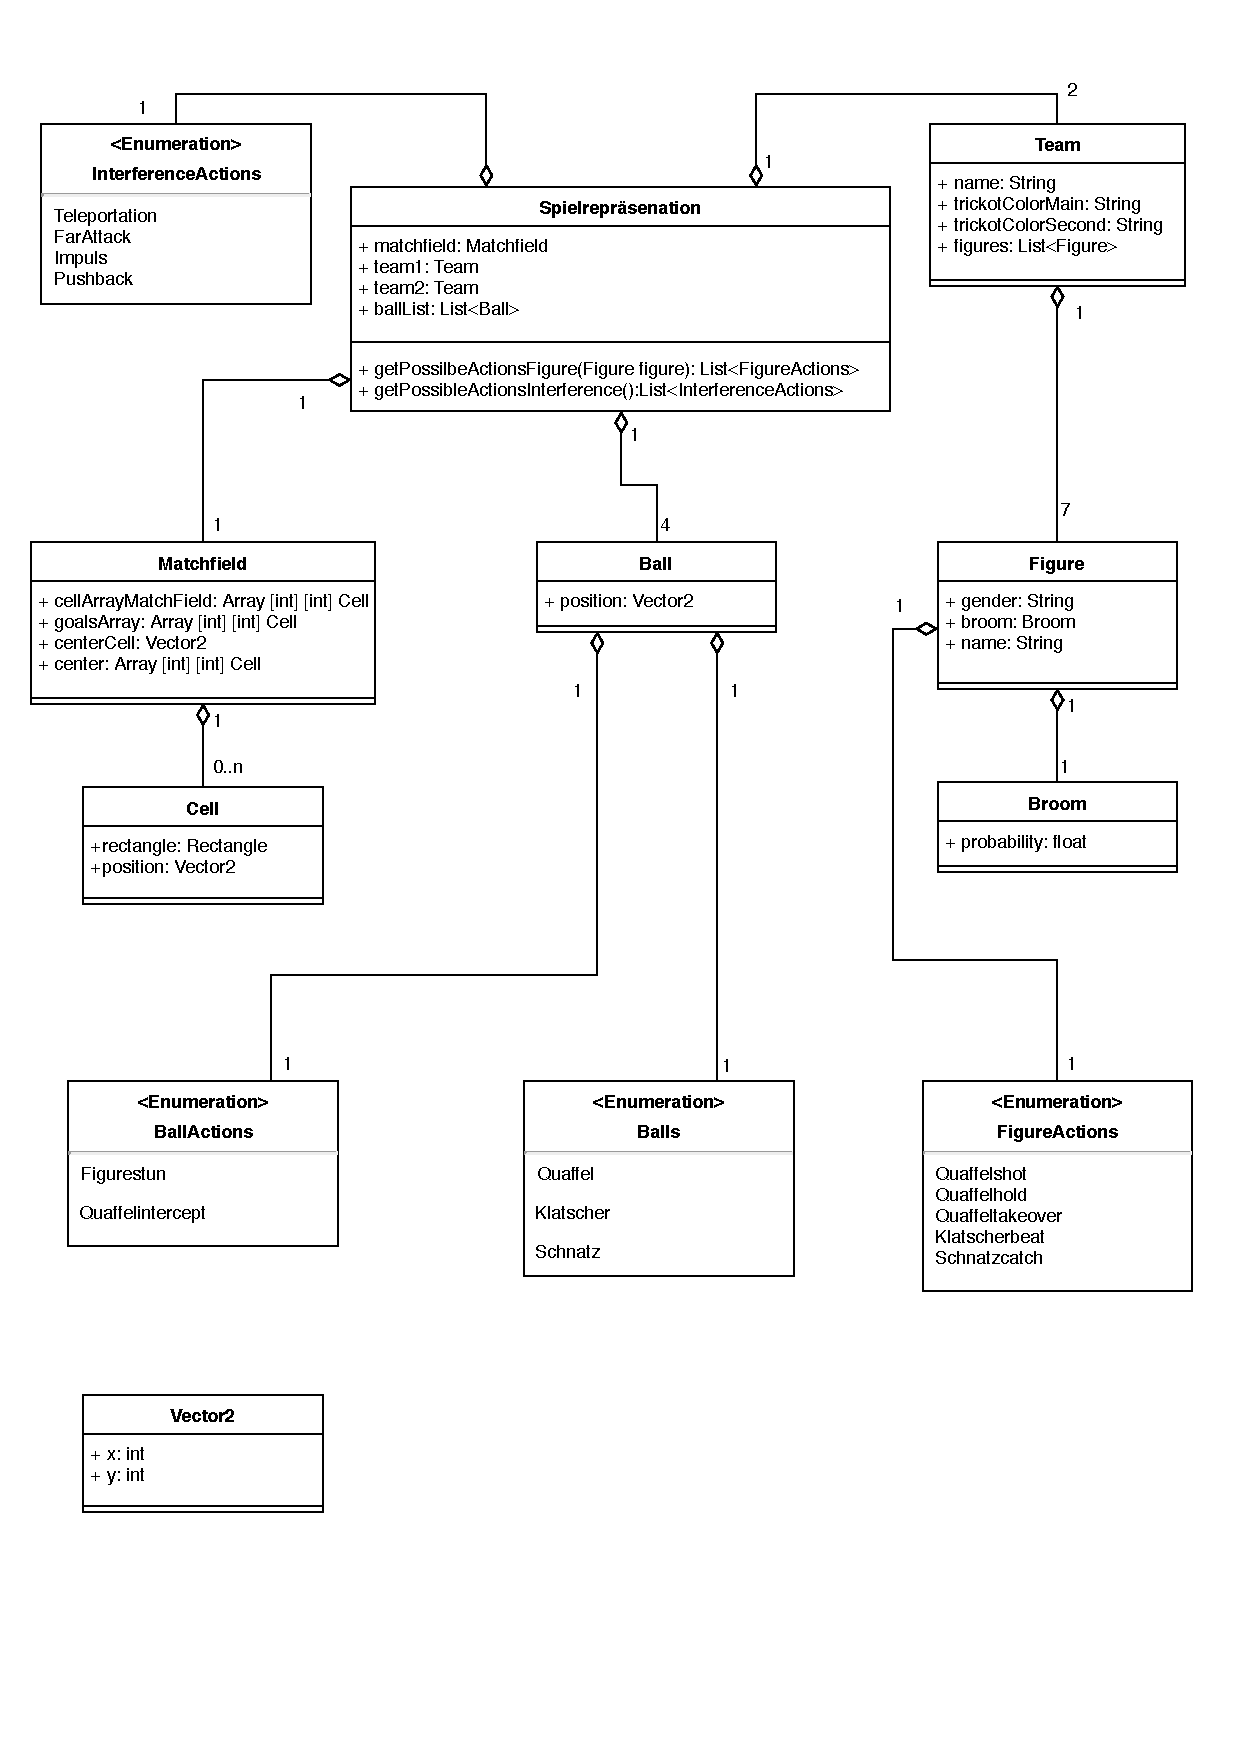
\includegraphics[scale=0.7]{images/model.pdf}
    \end{figure}

\subsection{Beschreibung}
	\subsubsection{Gamerepresentation (Klasse)}
	
		\begin{description}
                
			\item[Konstruktor (Methode)]
			Der Konstruktor erstellt eine Instance des Objektes Gamerepresentation. In diesem Objekt sind alle Objekte die für das Spiel notwendig sind und auf dem Spielfeld agieren enthalten und jeweils eine Instanz erstellt.
                
        	\item[getPossibleActionsFigure (Methode)]
        	Diese public Methode hat den Zweck eine Liste zu erstellen, in der alle möglichen Aktionen aufgelistet werden, die eine übergebene Spielfigur machen kann. Dazu überprüft die Methode welchen Typ Figur die übergeben Spielfigur hat, und welche AKtionen sie dadurch durchführen darf und gibt diese als Liste wieder.
        	
        	\item[getPossibleActionsInterference (Methode)]
        	Diese public Methode gibt die in der Enumeration definierten Einmischungen als Liste zurück. Dazu liest sie die Enumeration ein und spiechert diese in einer Liste, welche dann zurückgegeben wird. 
        \end{description}
        	
        \subsubsection{Matchfield (Klasse)}
        \begin{description}
        	\item[Konstuktor (Methode)]
        	In dem Konstruktor für das Matchfield, wird das eigentliche Spielfeld erstellt. Dazu erstellt diese Klasse ein Array von Zellen, welche das Spielfeld repräsentieren. Außerdem gibt es noch Bereiche, die besonders sind, aber auch Zellen auf dem Spielfeld sind. So sind die Torringe ebenfalls in einem Array hinterlegt, das Zentrum ist als Vektor hinterlegt und das Mittelfeld ist ebenfalls als Array hinterlegt.
        \end{description}
        
        \subsubsection{Team (Klasse}
        \begin{description}
        	\item[Konstruktor (Methode)]
        	Das Team ist ebenfalls Bestandteil der Klasse Gamerepresentation. In dem Team werden die 7 Spieler instantiiert, so wie der Name, die Trickotfarbe und die Ersatzfarbe für die Trickots.
        \end{description}
        
        \subsubsection{Ball (Klasse)}
        \begin{description}
        	\item[Konstuktor (Methode)]
        	Durch die Klasse Ball wird ebenfalls in der Gamerepresentation ein Bestandteil des Spieles instantiiert. Die Bälle bestehen aus einer Enumeration, welche Bälle es gibt, so wie aus einer Position, die als Vektor repräsentiert wird. Außerdem besitzt die Klasse Ball noch eine Enumeration, welche Aktionen ein Ball machen kann.
        \end{description}

\subsection{Zuordnung der Funktionalen Anforderungen}

Die Funktionalen Anforderungen werden den Methoden folgendermaßen zugeteilt:


\begin{table}[h]
	\centering
	\begin{tabular}{|l|l|}
    	\hline
    	\textbf{Methode} & \textbf{Funktionelle Anforderungen} \\ \hline
    	getPossibleActionsFigure		&	FA21, FA24, FA26, FA28, FA30\\ \hline
    	getPossibleActionsInterference	&	FA32 - FA35\\ \hline

	\end{tabular}
\end{table}